\documentclass[11pt,a4paper]{article}
\usepackage[margin=2.1cm]{geometry}
\usepackage[T1]{fontenc}
\usepackage[utf8]{inputenc}
\usepackage{lmodern}
\usepackage{booktabs}
\usepackage{array}
\usepackage{xcolor}
\usepackage{enumitem}
\usepackage{graphicx}
\usepackage{caption}
\usepackage{listings}
\usepackage{microtype}
\usepackage{hyperref}
\hypersetup{colorlinks=true,linkcolor=blue!55!black,urlcolor=blue!55!black}
\setlist{nosep,leftmargin=*}
\captionsetup{font=small,labelfont=bf}
\graphicspath{{figures/}}

\lstset{basicstyle=\ttfamily\footnotesize,frame=single,framesep=4pt,
        backgroundcolor=\color{black!3},rulecolor=\color{black!25},
        breaklines=true,columns=fullflexible,xleftmargin=0pt}

\newcommand{\modelcls}{\textsc{TomaNet-C}}
\newcommand{\modeldet}{\textsc{TomaNet-D}}
\newcommand{\tl}{\texttt{TomaLayer}}
\newcommand{\tb}{\texttt{TomaBlock}}

\title{\textbf{\tl{}: the Shared Building Block of TomaNet}\\[4pt]
\large What it does, what it takes, and how the same block builds both models}
\author{Tomato disease detection project}
\date{\today}

\begin{document}
\maketitle

\section{The idea in one paragraph}
TomaNet is built from one small unit, \tb{}. Stack \texttt{n} of those back to back and
you have a \tl{}. That is the whole abstraction: \tl{} is not a new kind of layer, it is
a repeat-counter around \tb{}. The interesting part is where it gets used --- the same
\tl{} code builds the four backbone stages that \modelcls{} and \modeldet{} \emph{share},
and the four extra fusion points that only \modeldet{} has. Nothing is re-implemented per
task; only the arguments change.

\begin{figure}[h]
  \centering
  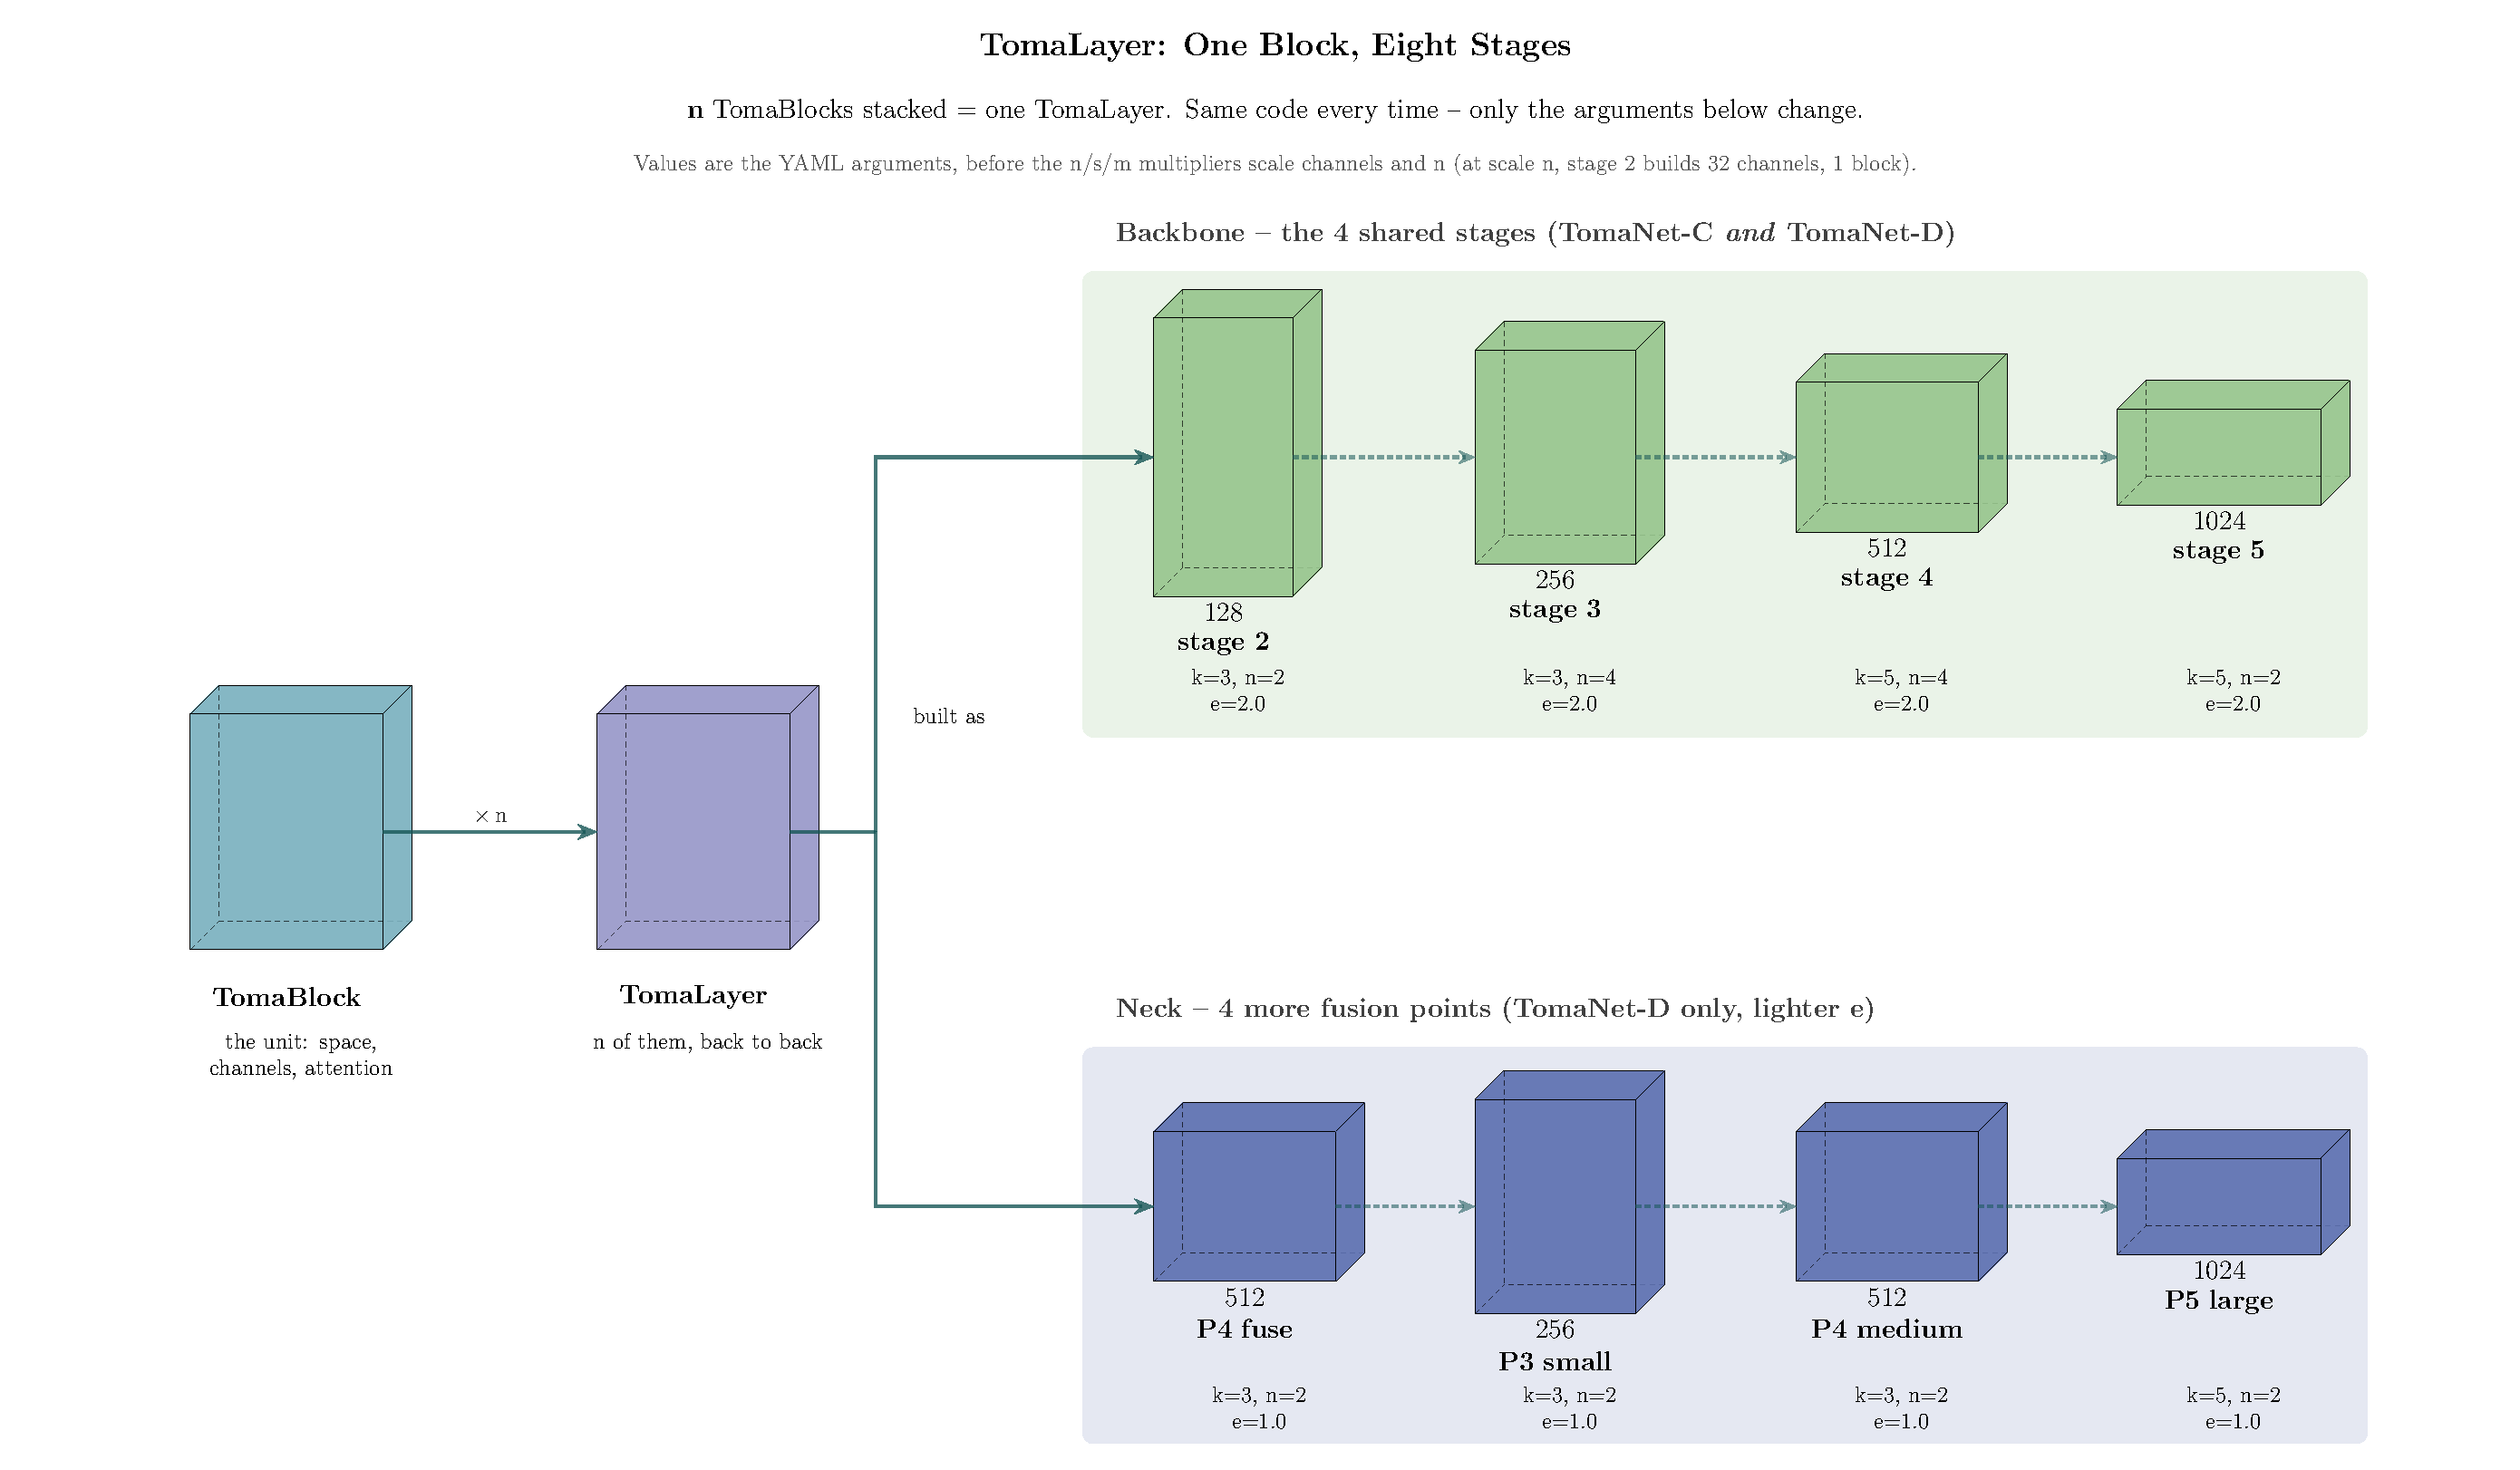
\includegraphics[width=0.92\linewidth]{fig_tomalayer_usage.pdf}
  \caption{One block, stacked into a \tl{}, then instantiated eight times: four shared
  backbone stages (green, in both models) and four neck fusion points (blue, \modeldet{}
  only). Tile height tracks feature-map size and tile width tracks channels, so the shape
  matches the real models; the values under each tile are the literal YAML arguments.}
\end{figure}

\section{Inside one \tb{}}
A \tb{} runs five steps in a fixed order, then optionally adds the input back. Written in
the order they execute (this is literally \texttt{TomaBlock.forward} in
\texttt{tomanet/modules.py}):

\begin{enumerate}
  \item \textbf{RepPConv (partial convolution, $3{\times}3$).} Convolves only the first
    quarter of the channels and passes the other three quarters straight through, then
    concatenates. Convolving fewer channels means less memory traffic, which is the real
    bottleneck on small devices --- not the arithmetic. At training time this step has
    three parallel branches ($3{\times}3$, $1{\times}1$, identity, each with its own
    BatchNorm); at deployment they collapse into a single $3{\times}3$ convolution.
  \item \textbf{$1{\times}1$ expand.} Widens the channels to
    \texttt{hidden = int(c1 $\times$ e)}, giving the next step room to work in.
  \item \textbf{Depthwise convolution, $k{\times}k$.} One filter per channel, so a larger
    $k$ costs almost nothing. This is the \emph{only} place $k$ is used.
  \item \textbf{CoordAtt (coordinate attention).} Pools along height and width separately,
    so the attention weights remember \emph{where} something is, not just which channel it
    was in. Lesions are small and position-specific, which is why plain channel-only
    attention (SE/ECA) was not used here.
  \item \textbf{$1{\times}1$ project.} Brings the channels back down to \texttt{c2}.
  \item \textbf{Residual add}, but only when \texttt{c1 == c2}. When the block changes the
    channel count there is nothing to add, so it is skipped automatically.
\end{enumerate}

\noindent The bottom row of Figure~\ref{fig:c} shows these steps as a chain.

\section{The parameters \tl{} takes}
\tl{} has seven arguments. Two are filled in for you, and in practice only three are ever
varied across the whole project.

\begin{center}
\small
\begin{tabular}{@{}llll@{}}
\toprule
\textbf{Argument} & \textbf{What it controls} & \textbf{Default} & \textbf{Used in TomaNet} \\
\midrule
\texttt{c1} & input channels & --- & filled in automatically from the previous layer \\
\texttt{c2} & output channels & --- & 128 / 256 / 512 / 1024, then width-scaled \\
\texttt{n}  & how many \tb{}s are stacked & 1 & 2 or 4, then depth-scaled \\
\texttt{k}  & kernel of the depthwise step & 3 & 3 in early stages, 5 in deep stages \\
\texttt{e}  & hidden width $=$ \texttt{c1}$\times$\texttt{e} & 2.0 & 2.0 in the backbone, 1.0 in the neck \\
\texttt{attn} & use CoordAtt (else identity) & \texttt{True} & \texttt{True} everywhere \\
\texttt{rep}  & use the 3-branch RepPConv & \texttt{True} & \texttt{True} everywhere \\
\bottomrule
\end{tabular}
\end{center}

\vspace{4pt}
\noindent Two details worth knowing:
\begin{itemize}
  \item Only the \emph{first} block in a \tl{} maps \texttt{c1}$\to$\texttt{c2}; the
    remaining \texttt{n}$-$1 blocks are \texttt{c2}$\to$\texttt{c2}, so they all get the
    residual connection.
  \item The quarter-of-the-channels split is \texttt{ratio=0.25} inside \tb{}. It is not
    exposed on \tl{}, because nothing in either model changes it.
\end{itemize}

\noindent In a model YAML one call site is a single line, where the number before the
module name is \texttt{n}:

\begin{lstlisting}
  - [-1, 4, TomaLayer, [256, 3]]        # n=4, c2=256, k=3, e defaults to 2.0
  - [-1, 2, TomaLayer, [512, 3, 1.0]]   # n=2, c2=512, k=3, e=1.0  (neck)
\end{lstlisting}

\section{How the same block plugs into both models}
Ultralytics has no plugin registry, so two small things make \tl{} usable from a YAML:

\begin{enumerate}
  \item \texttt{tomanet.register.register()} binds \tb{}, \tl{} and \texttt{CoordAtt} into
    the namespaces that the YAML parser resolves names against.
  \item \texttt{scripts/patch\_ultralytics.py} adds those names to the parser's
    channel-handling sets, so \texttt{c1}/\texttt{c2} are injected and the width multiplier
    is applied. Without the patch a model still builds, but the channels are not scaled ---
    so \texttt{verify\_setup.py} fails loudly if it is missing.
\end{enumerate}

\noindent After that, using the block in either model is just writing the line above into
\texttt{tomanet-cls.yaml} or \texttt{tomanet-det.yaml} under \texttt{configs/models/}.

\subsection*{\modelcls{} --- classification}
Stem (two strided convolutions) $\to$ four \tl{} stages $\to$ global average pool $\to$
one fully-connected layer. Layers 0--8 are the trunk.

\begin{figure}[h]
  \centering
  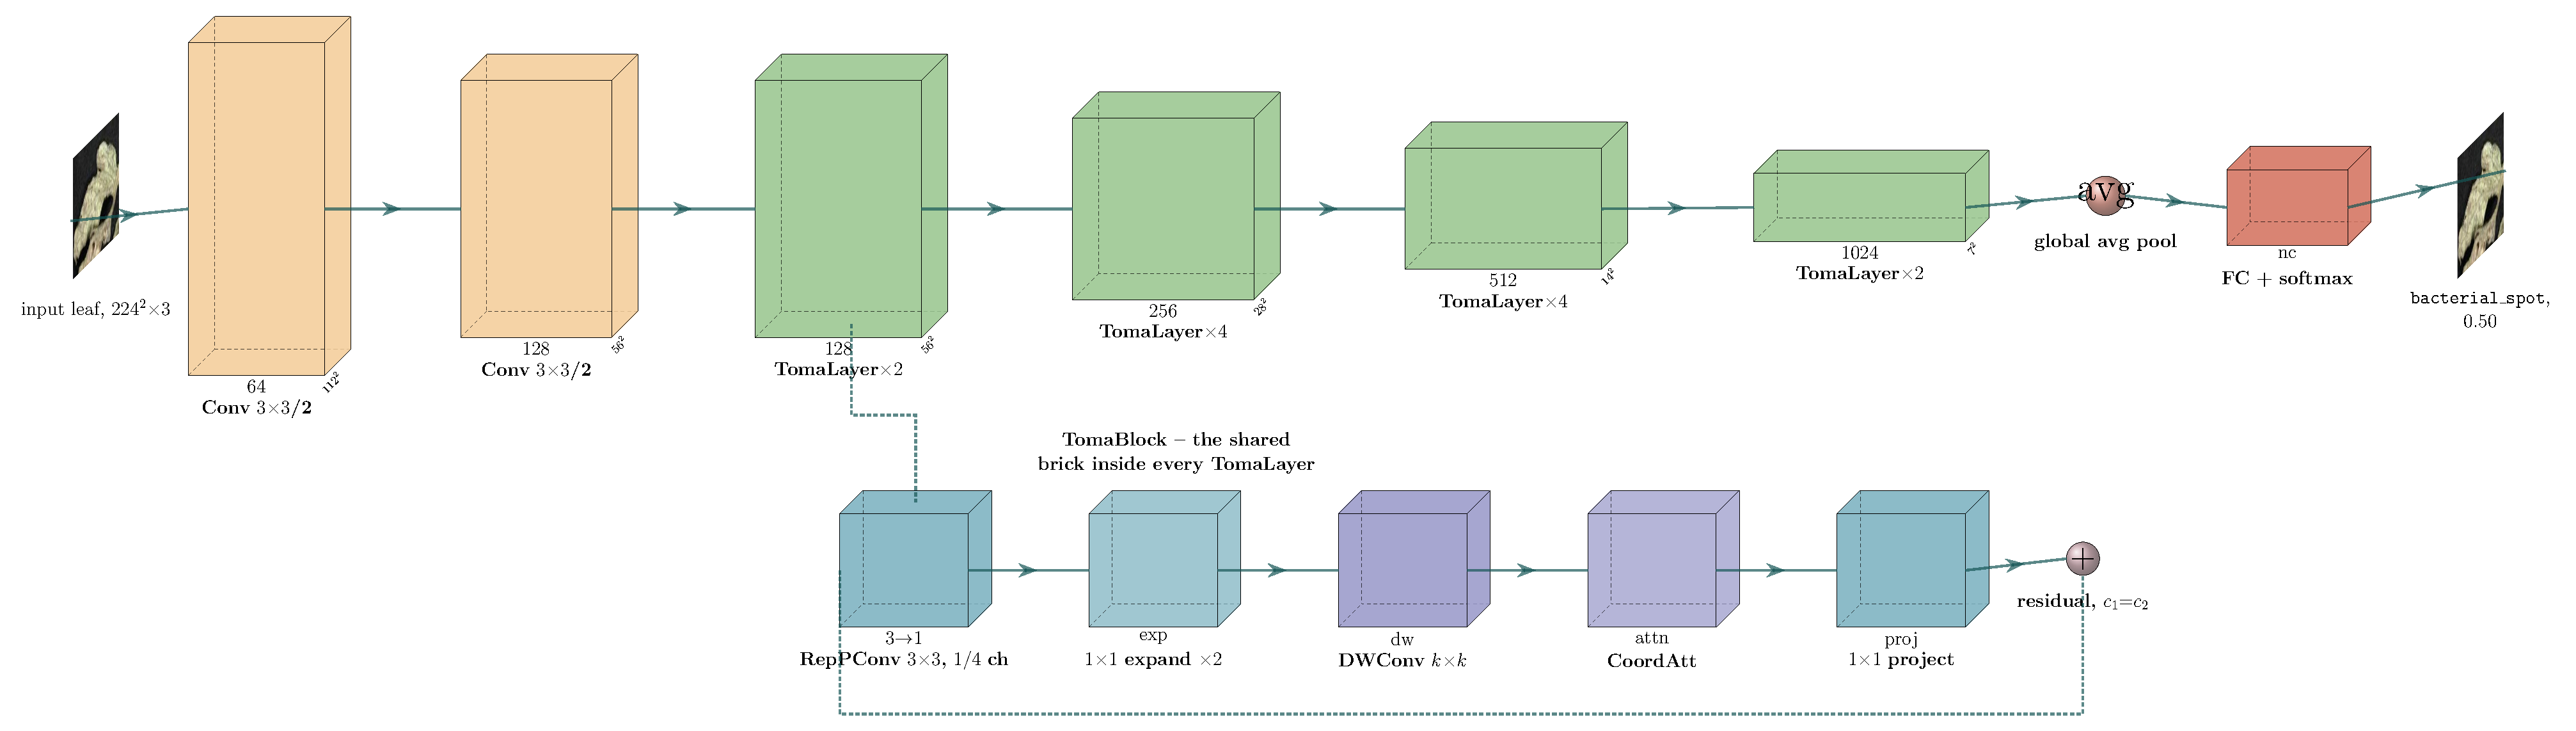
\includegraphics[width=\linewidth]{fig_tomanet_c.pdf}
  \caption{\modelcls{}. The bottom row is the \tb{} breakdown from Section~2.}
  \label{fig:c}
\end{figure}

\subsection*{\modeldet{} --- detection}
The same layers 0--8, byte for byte, then an SPPF block and a PAFPN neck that fuses three
resolutions, ending in three detect heads --- one each for small, medium and large objects.

\begin{figure}[h]
  \centering
  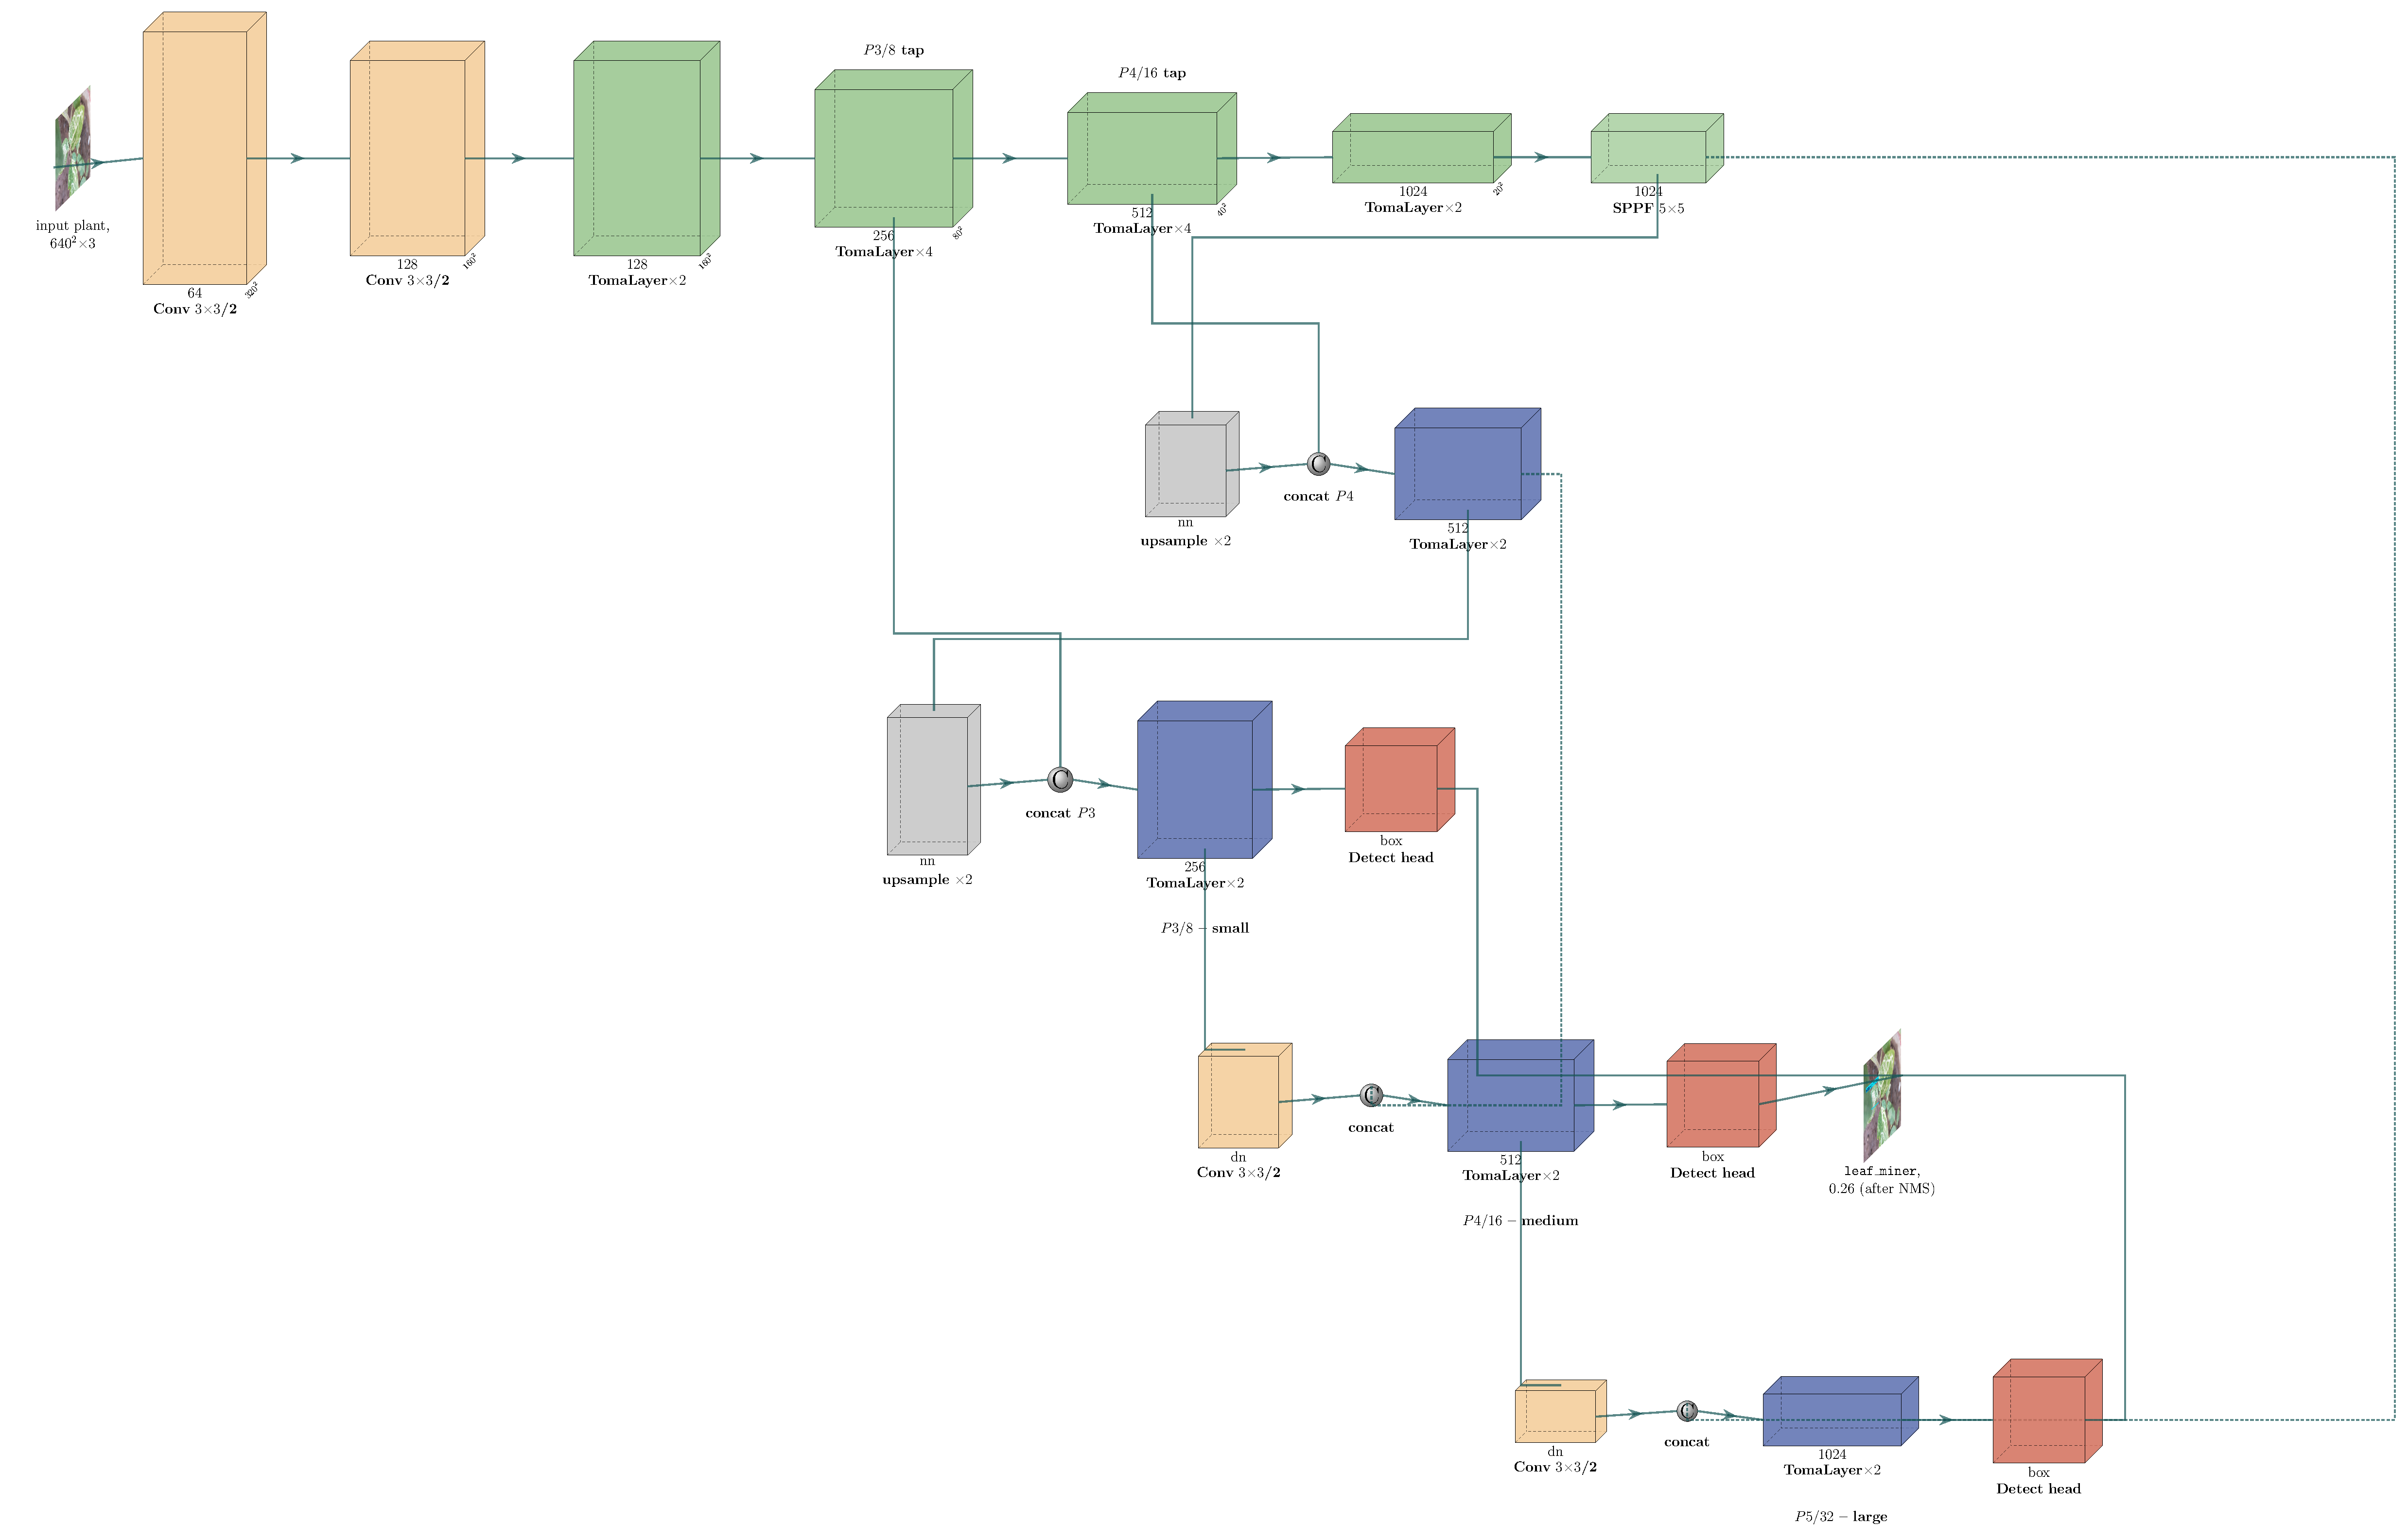
\includegraphics[width=\linewidth]{fig_tomanet_d.pdf}
  \caption{\modeldet{}. Everything green is the shared trunk; everything blue is the neck,
  which is where the four extra \tl{} calls live. Full-size version:
  \texttt{figures/fig\_tomanet\_d.pdf}.}
\end{figure}

\subsection*{All eight call sites}
\begin{center}
\small
\begin{tabular}{@{}lllllll@{}}
\toprule
\textbf{Where} & \textbf{Layer} & \texttt{c2} & \texttt{k} & \texttt{n} & \texttt{e} & \textbf{Present in} \\
\midrule
Backbone stage 2 & 2  & 128  & 3 & 2 & 2.0 & C and D \\
Backbone stage 3 & 4  & 256  & 3 & 4 & 2.0 & C and D \\
Backbone stage 4 & 6  & 512  & 5 & 4 & 2.0 & C and D \\
Backbone stage 5 & 8  & 1024 & 5 & 2 & 2.0 & C and D \\
\midrule
Neck, top-down $P4$ & 12 & 512  & 3 & 2 & 1.0 & D only \\
Neck, $P3$ (small)  & 15 & 256  & 3 & 2 & 1.0 & D only \\
Neck, $P4$ (medium) & 18 & 512  & 3 & 2 & 1.0 & D only \\
Neck, $P5$ (large)  & 21 & 1024 & 5 & 2 & 1.0 & D only \\
\bottomrule
\end{tabular}
\end{center}

\vspace{4pt}
\noindent \textbf{These are the YAML arguments, not the built model.} The width and depth
multipliers are applied on top, so at scale n stage~2 is actually built with 32 channels
and a single block, and at scale m with 96 channels and two blocks. The table above is
what you edit; Section~5 is what you get.

\vspace{2pt}
\noindent Because the first nine layers are identical in both YAMLs, a trunk trained on
classification can initialise the detector and vice versa. That is a property of the
files, not a claim --- an automated test compares the two layer lists.

\section{Why TomaNet is tunable}
Everything below was measured on this machine with
\texttt{scripts/verify\_setup.py} and by rebuilding modified configs; none of it is
estimated.

\subsection*{Size: the width and depth multipliers}
Each model ships in three sizes. The multipliers scale \texttt{c2} (width) and \texttt{n}
(depth) everywhere at once, so one number changes the whole network.

\begin{center}
\small
\begin{tabular}{@{}lcccc@{}}
\toprule
\textbf{Scale} & \textbf{depth $\times$} & \textbf{width $\times$} & \textbf{\modelcls{} @ 224px} & \textbf{\modeldet{} @ 640px} \\
\midrule
n & 0.50 & 0.25 & 1.32\,M / 0.37 GFLOPs & 2.92\,M / 8.58 GFLOPs \\
s & 0.50 & 0.50 & 4.47\,M / 1.32 GFLOPs & 10.64\,M / 29.68 GFLOPs \\
m & 1.00 & 0.75 & 14.44\,M / 4.56 GFLOPs & 30.79\,M / 82.84 GFLOPs \\
\bottomrule
\end{tabular}
\end{center}

\vspace{4pt}
\noindent For reference, the shared trunk alone at scale n is 0.97\,M parameters --- about
three quarters of the whole classifier. The neck and the three detect heads are what the
detector adds on top of it.

\subsection*{Cost: the expansion factor}
\texttt{e} is the cheapest knob in the model, because it sets the width of the most
expensive step. The neck runs at \texttt{e=1.0} rather than the default \texttt{2.0},
which is where most of the detector's savings come from:

\begin{center}
\small
\begin{tabular}{@{}lcc@{}}
\toprule
\textbf{\modeldet{} at scale n} & \textbf{Parameters} & \textbf{GFLOPs @ 640px} \\
\midrule
neck at \texttt{e=2.0} (the default)   & 3.60\,M & 10.32 \\
neck at \texttt{e=1.0} (what ships)    & 2.92\,M & 8.58 \\
\midrule
\textit{saved}                          & \textit{0.68\,M} & \textit{1.74} \\
\bottomrule
\end{tabular}
\end{center}

\noindent The backbone is untouched by this, so the trunk stays byte-identical to
\modelcls{}.

\subsection*{Accuracy features that are nearly free}
\begin{itemize}
  \item \textbf{CoordAtt} (\texttt{attn}). Turning it off everywhere in \modeldet{}-n takes
    the model from 2.92\,M to 2.84\,M parameters and from 8.58 to 8.57 GFLOPs --- roughly
    0.08\,M parameters and 0.01 GFLOPs for the whole network. It is kept on because the
    cost is that small.
  \item \textbf{RepPConv} (\texttt{rep}). Three branches at training time, one $3{\times}3$
    convolution after \texttt{fuse()}, so inference pays for one branch. The fold is exact
    to floating-point noise: the largest difference between the unfused and fused outputs
    is $2.4{\times}10^{-7}$.
  \item \textbf{Kernel size} (\texttt{k}). 3 in the early, high-resolution stages and 5 in
    the deep, low-resolution ones. Because the step is depthwise, the larger kernel buys a
    wider receptive field for almost no extra parameters.
\end{itemize}

\subsection*{What to edit, in practice}
\begin{itemize}
  \item \textbf{Need it smaller or larger?} Change the scale letter (\texttt{n}/\texttt{s}/\texttt{m}).
    Nothing else has to change.
  \item \textbf{Need it cheaper without shrinking the channels?} Lower \texttt{e} at
    specific call sites, as the neck already does.
  \item \textbf{Need more capacity in one place only?} Raise \texttt{n} on that one line.
  \item \textbf{Deploying?} Call \texttt{fuse\_reparam(model)} after loading weights so the
    three training branches collapse.
\end{itemize}

\noindent The scale-suffixed YAMLs
(\texttt{tomanet-clsn.yaml}, \texttt{tomanet-detn.yaml}, \dots) are regenerated from the
two base configs on every run, so edits belong in \texttt{tomanet-cls.yaml} and
\texttt{tomanet-det.yaml} only.

\end{document}
